\documentclass[a4paper]{cas-sc}

\usepackage{amsmath,amssymb,amsfonts}
\usepackage{amsthm}
\usepackage{algorithmic}
\usepackage{algorithm}
\usepackage{graphicx}
\usepackage{booktabs}
\usepackage{array}
\usepackage{tabularx}
\usepackage{multirow}
\usepackage{etoolbox}
\usepackage[authoryear]{natbib}
\usepackage{hyperref}

\newtheorem{definition}{Definition}
\newcommand{\hd}[1]{{\bfseries\boldmath #1}}
\AtBeginEnvironment{table}{\setlength{\belowcaptionskip}{4pt}}
\setlength{\emergencystretch}{1.5em}

% No author ORCID identifiers are listed in this anonymized manuscript.
\renewcommand{\printorcid}{}

\begin{document}

\shorttitle{BridgeSentry: Dual-Chain Fuzzing for Bridge Exploit Reconstruction}
\shortauthors{Anonymous}

\title[mode=title]{BridgeSentry: Reconstructing Cross-Chain Bridge Exploits with Dual-Chain Fuzzing and Execution-Only Validation}

\begin{abstract}
Cross-chain bridges have lost billions of US dollars to exploits whose root causes span a source-chain contract, an off-chain relay, and a destination-chain contract. Reproducing such an exploit requires executing all three domains together and judging the outcome from what actually executed. We present BridgeSentry, a fuzzing harness (a test environment that executes automatically generated inputs against target contracts) that reconstructs bridge exploits in two Ethereum Virtual Machine (EVM) instances joined by a relay. Its design extends Atomic Transfer Graphs (ATGs) with transfer-key invariants that evaluate asset conservation, authorization, and uniqueness per canonical key binding a source lock, its relay message, and its destination effect, and uses retrieval-augmented generation (RAG) over 48 documented incidents to produce attack scenarios that serve as initial inputs (seeds) of the search. We first show, for this harness, that the oracle, the procedure that decides whether an executed input is an exploit, can make such an evaluation meaningless: an earlier oracle of the harness, which derived its state from the generated scenario text, reported violations on all 12 fixtures (executable re-implementations of historical incidents) without executing target bytecode, reported none on the 11 deployable fixtures once restricted to execution-derived state, and still fired on a fixture of the Nomad incident whose root cause had been fixed. We therefore count a sequence of transactions (a trace) as a valid exploit only if addresses controlled by the adversary gain bridged assets in the token transfers committed on both chains, the trace replays, and the same trace gains nothing on a paired patched variant, a copy of the fixture in which the documented root cause is fixed. Under this criterion, on the two incidents evaluated so far, Nomad and Qubit, every vulnerable-variant run found a valid exploit and no patched-variant run raised an alert, in three rounds of five seeds and 20\,s each. Retrieval-generated seeds were faster than random seeds on Qubit but not on Nomad, so these small fixtures do not establish a benefit of semantic guidance. The evaluated configuration does not exercise the per-key authorization and uniqueness checkers, the distance-guided reward, or relay fault injection, and results for the remaining incidents and for ablations of individual modules are not reported.
\end{abstract}

\begin{keywords}
Cross-chain bridge security \sep Smart contract fuzzing \sep Transfer invariants \sep Atomic transfer graph \sep Exploit reconstruction \sep Retrieval-augmented generation
\end{keywords}

% The cas-sc front matter sets a 117pt-wide box internally; the warning is suppressed for the title block only.
{\hfuzz=120pt\maketitle}

\section{Introduction}\label{sec:intro}

Cross-chain bridges move assets and messages between otherwise isolated ledgers. A user locks or burns value on a source chain, an off-chain relay or validator set attests to the resulting event, and a contract on the destination chain mints or releases the corresponding value~\citep{belchior2021survey, augusto2024sok}. This construction concentrates value at the seams between three execution domains, and failures at those seams rank among the costliest incidents in decentralized finance (DeFi). Individual exploits have caused reported losses in the hundreds of millions of US dollars, led by Ronin (US\$624~million) and PolyNetwork (US\$611~million); Table~\ref{tab:losses} lists the costliest documented cases. Their root causes include compromised validator keys, faulty initialization of message verification, forged deposit events accepted by relays, and replayed messages~\citep{lee2023sok, duan2023attacks, liao2024smartaxe}.

\begin{table}[!t]
\centering
\caption{The costliest documented cross-chain bridge exploits, by reported loss. Figures are drawn from systematic reviews of bridge incidents~\citep{lee2023sok, augusto2024sok, zhang2024bridgesok}.}
\label{tab:losses}
\footnotesize
\begin{tabular*}{\linewidth}{@{\extracolsep{\fill}}lrr@{}}
\toprule
\hd{Incident} & \hd{Year} & \hd{Loss (US\$M)} \\
\midrule
Ronin Network   & 2022 & 624 \\
PolyNetwork     & 2021 & 611 \\
Wormhole        & 2022 & 326 \\
Nomad           & 2022 & 190 \\
Multichain      & 2023 & 126 \\
Harmony Horizon & 2022 & 100 \\
\bottomrule
\end{tabular*}
\end{table}

Recent work approaches bridge security from several directions. Static analyzers recover cross-chain data flows and external-interaction flaws from bridge contracts~\citep{liao2024smartaxe, zhou2025bridgeguard}. Monitors and transaction-graph detectors flag anomalous behavior in deployed bridges~\citep{augusto2025xchainwatcher, wu2025safeguarding, lin2025connector}, and an accounting-based analysis traces many bridge attacks to the absence of end-to-end value accounting~\citep{liu2024montecrypto}. BridgeFuzz brings fuzzing, the automated generation and execution of test inputs, to bridge deployments that include both on-chain contracts and off-chain relayers~\citep{winkler2026bridgefuzz}. In parallel, methods based on large language models (LLMs) now generate properties, invariants, and fuzzing seeds for single-chain contracts~\citep{liu2025propertygpt, wang2024smartinv, gai2026llama}.

Two obstacles remain when the goal is to execute a bridge exploit end to end and to know that it was executed. The first is the oracle, the procedure that decides whether an executed sequence of transactions (a trace) constitutes an exploit. A bridge failure is a broken relation among one source-chain lock, the relay message that attests to it, and one destination-chain effect. An aggregate balance check lets an excess lock by one user mask an unauthorized mint to another, and an authorization check that only requires some earlier deposit is satisfied by an unrelated transfer. The second is guidance and measurement. A fuzzer derives new test inputs by randomly modifying (mutating) earlier ones; exploit sequences cross three domains in a fixed causal order, which can make them hard to reach for mutation driven by randomness or code coverage alone, and a campaign that counts a success whenever an invariant fires cannot tell whether the vulnerable path ran at all.

The design of BridgeSentry rests on one observation: every bridge transfer carries a canonical key, assembled from the bridge instance, the source and destination domains, the emitter, the nonce, and the transferred asset, amount, recipient, and payload, and several documented exploit classes, such as forged deposits, unproven messages, and replayed messages, violate a predicate over the records that share such a key. The design makes this key the unit of both the oracle and the guidance. It extends Atomic Transfer Graphs (ATGs)~\citep{dubler2025atg}, a formalism that models a cross-chain protocol as a labeled graph of asset transfers and messages, with key-indexed conservation, authorization, and uniqueness invariants. It compiles the invariants into checkers, defines for the conservation invariant a distance to its violation boundary, and evaluates the checkers over a global state that joins two Ethereum Virtual Machine (EVM) instances and a controllable relay. Retrieval-augmented generation (RAG), in which an LLM generates text conditioned on entries retrieved from a knowledge base, draws on 48 documented incidents to supply attack scenarios and semantic waypoints, intermediate objectives intended to steer mutation toward the invariant boundaries. A capability matrix admits relay tampering or replay only when an incident's documented root cause grants that power to the adversary.

Evaluating such a harness raises a measurement problem that precedes any comparison. An earlier oracle of BridgeSentry derived its state from the text of the generated scenarios. We evaluated it on 12 fixtures, each an executable re-implementation of the contracts involved in one historical incident: it reported invariant violations on all 12 when no target bytecode ran, on none of them when only execution-derived state was visible, and on a Nomad fixture whose root cause had been patched. A trigger rate computed with such an oracle measures the scenario generator, not the exploit. We therefore evaluate with an execution-only oracle and, for each fixture, a paired patched variant, that is, a copy of the fixture in which the documented root cause is fixed. We report only what this criterion supports: valid exploits on the vulnerable variants and no alerts on the patched variants of the two incidents evaluated so far, Nomad and Qubit. The evaluated configuration uses the retrieval-generated scenarios as initial seeds for coverage-guided mutation; the remaining design components are described but not yet evaluated.

The contributions of this paper are as follows.
\begin{itemize}
    \item We formalize transfer-key invariants for cross-chain bridges, an extension of ATGs in which asset conservation, authorization, and uniqueness are evaluated per canonical transfer key, together with a distance for the conservation invariant that is zero exactly when the invariant is violated and decreases monotonically as a safe state approaches the violation boundary. These definitions are a design contribution; the configuration evaluated in this paper does not exercise their checkers.
    \item We design BridgeSentry, a fuzzing harness that runs two EVM instances joined by a relay, seeds its search with attack scenarios generated from retrieved incidents, captures and restores both EVM instances and the relay as a single global snapshot, and confines relay tampering and replay to the capabilities that each incident's root cause grants. The evaluated configuration exercises the scenario seeds, dual-EVM execution with faithful relay delivery, and global snapshot restoration (Section~\ref{sec:evaluated}).
    \item We show on the 12 fixtures of an earlier configuration of our harness that its oracle, which derived its state from generated scenario text, made the invariant-trigger rate uninformative, and we define a valid-exploit criterion based only on executed token transfers, replay, and a paired patched variant. Under this criterion, BridgeSentry finds a valid exploit in every vulnerable-variant run and raises no alert in any patched-variant run of the two incidents evaluated so far.
\end{itemize}

The remainder of this paper is organized as follows. Section~\ref{sec:related} positions BridgeSentry against prior work. Section~\ref{sec:problem} defines the execution model, transfer-key invariants, threat model, and reconstruction outcomes. Section~\ref{sec:method} presents the three modules of BridgeSentry. Section~\ref{sec:experiments} reports the evaluation, Section~\ref{sec:discussion} discusses what the results imply for bridge testing, and Section~\ref{sec:conclusion} concludes.

\section{Related Work}\label{sec:related}

\subsection{Cross-chain bridge security}

Surveys and systematizations establish the attack surface of bridges. \citet{belchior2021survey} survey blockchain interoperability, \citet{augusto2024sok} systematize the security and privacy of 34 interoperability systems, \citet{zhang2024bridgesok} map bridge attack surfaces to defenses and open problems, and \citet{lee2023sok}, \citet{duan2023attacks}, and \citet{li2025blockchain} classify bridge hacks and defense approaches by protocol layer and root cause.

Analysis tools fall into three groups. Static analyzers inspect contract code: SmartAxe builds cross-chain data-flow graphs with taint rules tailored to bridge contracts~\citep{liao2024smartaxe}, BridgeGuard applies symbolic data-flow analysis with heuristic pruning to bridge router contracts~\citep{zhou2025bridgeguard}, and both build on general frameworks such as Slither~\citep{feist2019slither}. Monitors and detectors work on observed executions: XScope matches rule-based attack patterns on event logs~\citep{zhang2022xscope}, HighGuard checks cross-chain business-logic conformance at runtime~\citep{eshghie2024highguard}, XChainWatcher identifies anomalies in deployed bridges~\citep{augusto2025xchainwatcher}, and a second system also named BridgeGuard models attack transactions as graphs~\citep{wu2025safeguarding}, an approach that BridgeShield extends to heterogeneous graphs in a recent preprint~\citep{lin2025bridgeshield}. Traceability tools associate source-chain and destination-chain transactions~\citep{lin2025connector, lin2025track, zheng2024xsema}, including an LLM-assisted association method in a recent preprint~\citep{liang2025connex}. \citet{liu2024montecrypto} argue in a preprint that explicit end-to-end value accounting would prevent a broad class of bridge attacks, a view that the per-transfer conservation invariant of Section~\ref{sec:problem} operationalizes as a test oracle. GoAT-X structures LLM-based auditing of cross-chain token transfers around statically extracted constraints~\citep{feng2026goatx}.

Dynamic testing of bridges is the closest line of work. BridgeFuzz fuzzes bridge deployments that include on-chain contracts and off-chain relayers and reports balance mismatches, protocol errors, and off-chain denial of service~\citep{winkler2026bridgefuzz}. IntentFuzz, a concurrent preprint, recovers intent structures from intent-based bridges and fuzzes their fill and settlement functions~\citep{augusto2026intentfuzz}. The design of BridgeSentry differs from both in what drives and judges the search: its oracle evaluates conservation, authorization, and uniqueness per canonical transfer key over a joint snapshot of both chains and the relay, its guidance comes from retrieved incident knowledge rather than from coverage alone, and its relay faults are admitted only under an explicit per-fixture capability. The configuration evaluated in this paper implements only part of this design (Section~\ref{sec:evaluated}).

\subsection{Smart contract fuzzing}

Snapshot-based fuzzing made stateful exploration of contracts practical. ItyFuzz reuses snapshots to backtrack cheaply~\citep{shou2023ityfuzz}, and SmartShot mutates snapshots directly to reach hidden states~\citep{liang2025smartshot}. VulSEye directs graybox fuzzing toward statically identified targets~\citep{liang2025vulseye}, xFuzz uses learned models to prioritize cross-contract paths~\citep{xue2024xfuzz}, and execution on graphics processing units raises fuzzing throughput~\citep{chen2024gpufuzzing}. Profit-oriented fuzzers search for exploits that extract value~\citep{ye2024midas, kong2025fuzzing}, and an empirical comparison of contract fuzzers documents how strongly results depend on benchmark and configuration~\citep{wu2024fuzzers}, echoing earlier guidance on sound fuzzer evaluation~\citep{klees2018evaluating}. Domain-specific waypoints, introduced by FuzzFactory, let a fuzzer reward progress toward a goal other than coverage~\citep{padhye2019fuzzfactory}; BridgeSentry's semantic waypoints apply this idea to cross-chain predicates. All of these fuzzers execute a single chain, so none of them can execute the relay step through which a cross-chain bridge exploit passes from one chain to the other.

\subsection{Language models and retrieval for contract security}

LLMs now assist each stage of contract analysis. GPTScan combines reasoning by generative pre-trained transformer (GPT) models with program analysis to find logic vulnerabilities~\citep{sun2024gptscan}, a multi-agent system coordinates several LLM roles for end-to-end detection~\citep{wei2025advanced}, and ParaVul runs LLM reasoning and retrieval in parallel~\citep{huang2026paravul}. PropertyGPT retrieves reference properties to generate verifiable specifications~\citep{liu2025propertygpt}, while SmartInv and INVCON+ infer invariants through multimodal learning and verification, respectively~\citep{wang2024smartinv, liu2025invcon}. On the dynamic side, LLM4Fuzz uses an LLM to prioritize fuzzing targets~\citep{shou2024llm4fuzz}, LLAMA generates seeds under multiple feedback signals~\citep{gai2026llama}, CrossGuard adapts LLM guidance at runtime for cross-contract fuzzing~\citep{ali2025crossguard}, and PromFuzz combines LLM-driven and bug-oriented analysis~\citep{lin2025promfuzz}. LLM guidance has also been applied to network protocol fuzzing~\citep{meng2024llmguided}, price-oracle manipulation~\citep{gao2026airaclex}, access-control flaws~\citep{chen2026trace}, and attack synthesis against deep DeFi logic~\citep{wen2024foray}. BridgeSentry uses LLMs offline, to extract protocol semantics and to turn retrieved incidents into attack scenarios, and makes no LLM call inside the fuzzing loop.

\subsection{Formal models and graph representations}

Atomic Transfer Graphs model cross-chain protocols as labeled transfer graphs for secure-by-construction design~\citep{dubler2025atg}. BridgeSentry applies the formalism in the opposite direction, to derive testable invariants from existing bridge implementations. Execution property graphs unify control flow, data flow, and runtime state for contract analysis~\citep{qin2025epg}, and graph neural networks detect vulnerability patterns from contract structure~\citep{zhuang2020smart, liu2023gnn}.

Table~\ref{tab:rw-positioning} summarizes the most closely related tools in chronological order.

\begin{table*}[!t]
\centering
\caption{Representative tools in chronological order. Rows are ordered by year and, within a year, by first-author surname. Approach: static analysis, runtime or transaction monitoring, transaction tracing, graph learning, verification, fuzzing, or LLM-based auditing. Cross-domain: the tool executes source-chain, relay, and destination-chain logic together. LLM role: the task assigned to the language model. Works marked with a dagger are unreviewed preprints.}
\label{tab:rw-positioning}
\footnotesize
\setlength{\tabcolsep}{4pt}
\begin{tabularx}{\textwidth}{@{}>{\raggedright\arraybackslash}X>{\raggedright\arraybackslash}p{2.05cm}>{\raggedright\arraybackslash}p{1.75cm}>{\centering\arraybackslash}p{1.35cm}>{\centering\arraybackslash}p{1.35cm}>{\raggedright\arraybackslash}p{2.0cm}>{\centering\arraybackslash}p{1.25cm}@{}}
\toprule
\hd{Tool} & \hd{Venue and year} & \hd{Approach} & \hd{Bridge-specific} & \hd{Cross-domain} & \hd{LLM role} & \hd{Retrieval} \\
\midrule
XScope~\citep{zhang2022xscope} & ASE 2022 & Monitoring & Yes & No & None & No \\
ItyFuzz~\citep{shou2023ityfuzz} & ISSTA 2023 & Fuzzing & No & No & None & No \\
HighGuard~\citep{eshghie2024highguard} & ASE 2024 & Monitoring & Yes & No & None & No \\
SmartAxe~\citep{liao2024smartaxe} & FSE 2024 & Static & Yes & No & None & No \\
LLM4Fuzz$^\dagger$~\citep{shou2024llm4fuzz} & arXiv 2024 & Fuzzing & No & No & Guidance & No \\
GPTScan~\citep{sun2024gptscan} & ICSE 2024 & Static & No & No & Detection & No \\
Midas~\citep{ye2024midas} & ISSTA 2024 & Fuzzing & No & No & None & No \\
CrossGuard~\citep{ali2025crossguard} & CCPE 2025 & Fuzzing & No & No & Guidance & No \\
XChainWatcher~\citep{augusto2025xchainwatcher} & Middleware 2025 & Monitoring & Yes & No & None & No \\
ConneX$^\dagger$~\citep{liang2025connex} & arXiv 2025 & Tracing & Yes & No & Association & No \\
SmartShot~\citep{liang2025smartshot} & FSE 2025 & Fuzzing & No & No & None & No \\
VulSEye~\citep{liang2025vulseye} & TIFS 2025 & Fuzzing & No & No & None & No \\
BridgeShield$^\dagger$~\citep{lin2025bridgeshield} & arXiv 2025 & Graph & Yes & No & None & No \\
PropertyGPT~\citep{liu2025propertygpt} & NDSS 2025 & Verification & No & No & Properties & Yes \\
BridgeGuard, graph~\citep{wu2025safeguarding} & WWW 2025 & Graph & Yes & No & None & No \\
BridgeGuard, symbolic~\citep{zhou2025bridgeguard} & TDSC 2025 & Static & Yes & No & None & No \\
GoAT-X$^\dagger$~\citep{feng2026goatx} & arXiv 2026 & LLM auditing & Yes & No & Auditing & No \\
LLAMA~\citep{gai2026llama} & TIFS 2026 & Fuzzing & No & No & Seeds & No \\
ParaVul~\citep{huang2026paravul} & TIFS 2026 & Static & No & No & Detection & Yes \\
BridgeFuzz~\citep{winkler2026bridgefuzz} & EuroSec 2026 & Fuzzing & Yes & Yes & None & No \\
This work & 2026 & Fuzzing & Yes & Yes & Extraction, scenarios & Yes \\
\bottomrule
\end{tabularx}
\end{table*}

\section{Problem Formulation}\label{sec:problem}

\subsection{Cross-chain execution model}

A cross-chain bridge protocol $\mathcal{B}$ spans three execution domains: a source chain $\mathcal{C}_S$, a destination chain $\mathcal{C}_D$, and an off-chain relay $\mathcal{R}$. A transfer proceeds in three stages.
\begin{enumerate}
    \item A user $u$ invokes the deposit function of the source router contract $RC_S \in \mathcal{C}_S$, which calls the token contract $TC_S$ to lock assets of value $v$ and emits a deposit event $e_{\text{dep}}$.
    \item The relay $\mathcal{R}$ observes $e_{\text{dep}}$, validates it against the source-chain state, and transmits a message $m$ to the destination chain.
    \item The destination router contract $RC_D \in \mathcal{C}_D$ verifies $m$ under the bridge's rules and calls the token contract $TC_D$ to mint or release value $v$ to the recipient.
\end{enumerate}

\subsection{Atomic transfer graphs}

We model a bridge with the Atomic Transfer Graph formalism of \citet{dubler2025atg}, adapted to existing bridge implementations.

\begin{definition}[Atomic Transfer Graph]\label{def:atg}
An ATG is a directed labeled graph $G = (N, A, \Lambda)$ in which $N = N_U \cup N_C \cup N_R$ contains user accounts $N_U$, smart contracts $N_C$, and relay components $N_R$; $A \subseteq N \times N$ contains arcs that represent asset transfers or message transmissions; and $\Lambda: A \rightarrow \{\text{lock}, \text{unlock}, \text{mint}, \text{burn}, \text{relay}, \text{verify}\}$ labels each arc. Protocol invariants $\Phi = \{\phi_1, \ldots, \phi_k\}$ are defined over the graph and the states of its nodes.
\end{definition}

\subsection{Transfer keys and invariants}

The invariants of BridgeSentry are indexed by the identity of an individual transfer rather than evaluated over aggregate balances.

\begin{definition}[Canonical transfer key]\label{def:key}
The canonical transfer key of a transfer is the tuple
\begin{equation*}
\begin{aligned}
\kappa = (&\text{bridge instance}, \text{source domain}, \text{destination domain}, \text{emitter}, \text{nonce},\\
&\text{token}, \text{amount}, \text{recipient}, \text{payload hash}),
\end{aligned}
\end{equation*}
restricted to the fields that the protocol defines. $\mathcal{K}$ denotes the set of keys observed in an execution.
\end{definition}

The key binds a lock arc $a_l$, a relay arc $a_r$, and a mint or release arc $a_m$ to the same transfer through the predicate $\text{sameMsg}(a_l, a_r, a_m)$, which holds when the three arcs carry the same key. On this basis we define four invariant classes.

\paragraph{Asset conservation per transfer}
For every key $\kappa$, the value minted or released on $\mathcal{C}_D$ must not exceed the value locked on $\mathcal{C}_S$ after fees and documented tolerances:
\begin{equation}\label{eq:conservation}
    M_{\kappa}(\sigma) \leq L_{\kappa}(\sigma) - f_{\kappa} + \delta_{\kappa},
\end{equation}
where $L_{\kappa}$, $M_{\kappa}$, $f_{\kappa}$, and $\delta_{\kappa}$ are the locked value, the minted or released value, the fee, and the documented numerical tolerance of transfer $\kappa$ in state $\sigma$. Fee, rebase, and fee-on-transfer adjustments are admitted only when a fixture supplies a deterministic, protocol-specific accounting rule; assets without such a rule are excluded rather than assigned a zero adjustment. Indexing by $\kappa$ prevents an excess lock by one user from offsetting an unauthorized mint to another; aggregate balances serve only as diagnostics.

\paragraph{Authorization per message}
Every mint on $\mathcal{C}_D$ must be preceded by a deposit and a relay verification of the same transfer:
\begin{equation}\label{eq:authorization}
    \forall a_m \in A_{\text{mint}}\ \exists a_l \in A_{\text{lock}},\ a_r \in A_{\text{relay}} : \text{sameMsg}(a_l, a_r, a_m) \land (a_l \prec a_r \prec a_m),
\end{equation}
where $\prec$ denotes causal order. Binding the three arcs by key prevents an unrelated earlier deposit from satisfying the causal order.

\paragraph{Uniqueness per message}
Each key is consumed at most once on the destination chain:
\begin{equation}\label{eq:uniqueness}
    \forall \kappa \in \mathcal{K}: \text{consume\_count}(\kappa) \leq 1.
\end{equation}
Nonce uniqueness across deposit events is necessary but not sufficient, because a replayed relay delivery preserves the nonce and violates Eq.~\eqref{eq:uniqueness}.

\paragraph{Timeliness as a protocol-specific policy}
For a bridge whose specification defines a timeout $\tau_S$ and a refund path, any lock that is not completed within $\tau_S$ must become refundable:
\begin{equation}\label{eq:timeliness}
    \forall a_l \in A_{\text{lock}}: \bigl(t_S^{\text{now}} - t_S(a_l) > \tau_S\bigr) \Rightarrow \text{refundable}(a_l).
\end{equation}
Intent-based systems, liquidity bridges, and canonical mint-and-burn bridges intentionally provide no refund after finality, so Eq.~\eqref{eq:timeliness} is instantiated only for bridges whose specification defines a refund path.

\subsection{Threat model}

The adversary $\mathcal{A}$ is rational and can deploy and call arbitrary contracts on $\mathcal{C}_S$ and $\mathcal{C}_D$, submit transactions with crafted inputs to bridge contracts, observe all public events and relay messages, and exploit timing differences between the chains, including block-production delays and finality asymmetries. The adversary cannot break the consensus of either chain or the underlying cryptographic primitives.

Off-chain incidents such as compromised validator keys require a further distinction between what the adversary does and what the harness injects. We encode this distinction explicitly.

\begin{definition}[Capability matrix]\label{def:capability}
For a benchmark fixture $F$, the capability matrix $C_F \in \{0,1\}^{2}$ records whether the documented root cause of $F$ grants the adversary the power to tamper with relay messages and the power to replay them. A relay tampering or replay action is admissible in a run on $F$ only if the corresponding entry of $C_F$ is one, and a resulting trace counts as an exploit only if the target protocol's own verification code accepts the message.
\end{definition}

\subsection{Reconstruction problem and outcomes}

A fixture $F$ consists of target contracts $T_F$ that reproduce the vulnerable logic of a historical incident, together with the invariant $\phi_F \in \Phi$ that the documented exploit violates. $T_F$ is either the deployed contracts on forks of the affected chains at a block preceding the attack or, as for the fixtures evaluated in this paper, a minimal re-implementation of the documented root cause deployed on an empty chain state. A trace is a sequence of actions on $\mathcal{C}_S$, $\mathcal{R}$, and $\mathcal{C}_D$.

\begin{definition}[Reconstruction outcomes]\label{def:outcomes}
A trace $s$ on fixture $F$ is a trigger if the final global state $\sigma$ violates $\phi_F$. A trigger is bytecode-backed if $s$ executes at least one basic block, a straight-line sequence of instructions with a single entry and a single exit, of $T_F$ without an early revert and causes a material change of state, and it is hollow if it executes no basic block of $T_F$.
\end{definition}

Definition~\ref{def:outcomes} makes explicit a distinction that a trigger count hides: a hollow trigger satisfies the oracle without exercising the vulnerable code, so it reconstructs nothing. A bytecode-backed trigger is, however, only as meaningful as the state on which $\phi_F$ is evaluated; Section~\ref{sec:rq-oracle} reports an oracle whose triggers were bytecode-backed and yet independent of the executed code. We therefore require a stronger outcome.

\begin{definition}[Valid exploit]\label{def:valid}
Let fixture $F$ have a paired patched variant $F'$ that differs from $F$ only in the fix of the documented root cause. A trace $s$ is a valid exploit on $F$ if (i) it executes code of $T_F$ and changes state; (ii) it uses only actions admissible under $C_F$; (iii) its gain reaches the adversary through a release or mint entry point of the protocol or through the relay; (iv) replaying $s$ from the same initial snapshot yields the same gains; (v) at the end of $s$, the addresses controlled by the adversary hold a positive net gain of at least one bridged asset, computed from the token transfers committed on both chains; and (vi) executing $s$ on $F'$ yields no such gain.
\end{definition}

Given $F$, $F'$, and $C_F$, the reconstruction problem is to find a valid exploit. Condition~(v) is an adversary-side counterpart of Eq.~\eqref{eq:conservation}: it does not reconstruct transfer keys, and it detects only violations that move bridged value to the adversary.

\section{BridgeSentry}\label{sec:method}

BridgeSentry consists of three modules that run in sequence: semantic extraction, retrieval-augmented scenario generation, and synchronized dual-chain fuzzing. Figure~\ref{fig:architecture} shows the architecture.

\begin{figure}
\centering
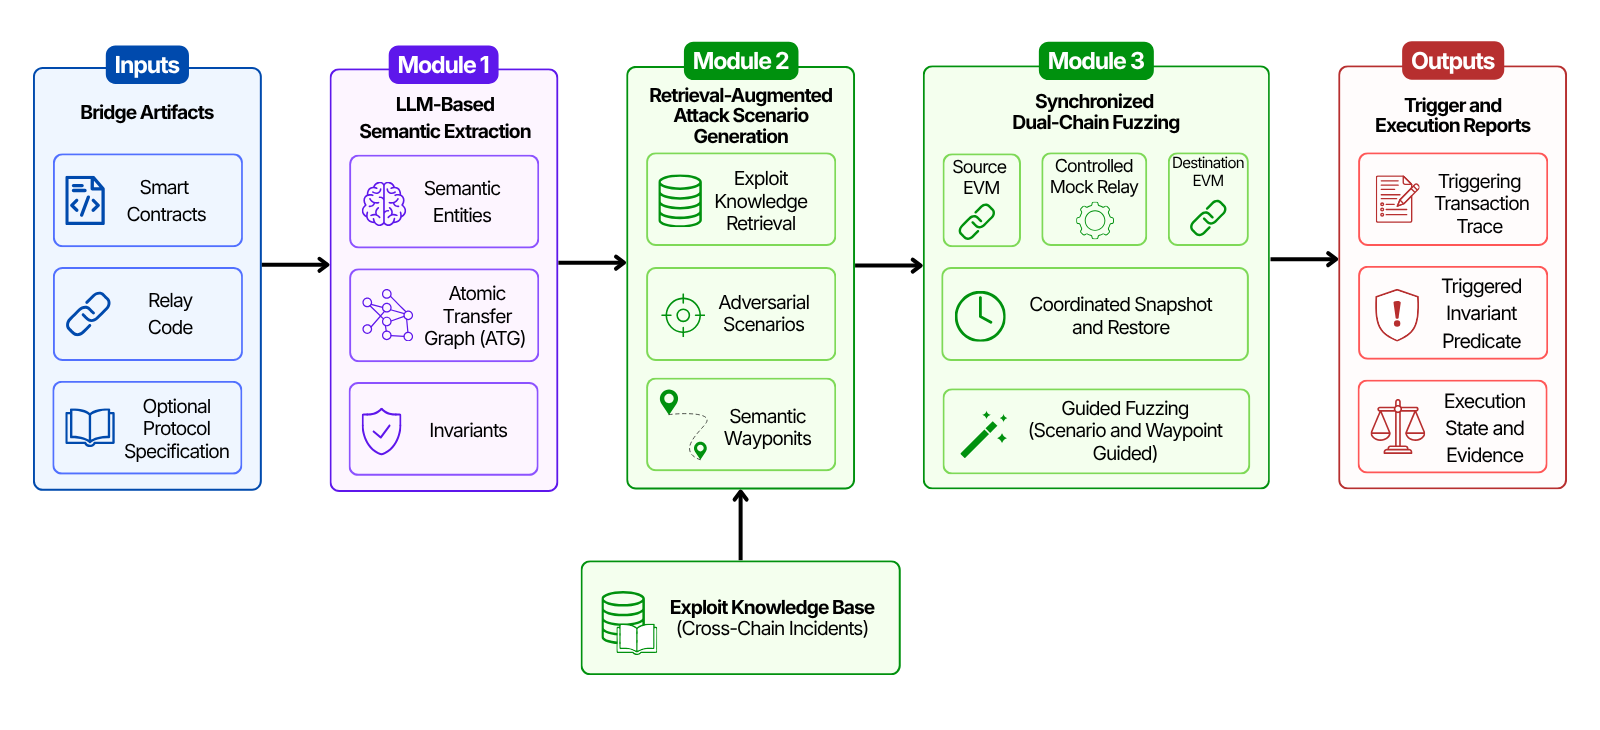
\includegraphics[width=\linewidth]{fig_architecture.png}
\caption{Architecture of BridgeSentry. Module~1 extracts an Atomic Transfer Graph and transfer-key invariants from bridge artifacts. Module~2 retrieves documented incidents and generates attack scenarios with semantic waypoints. Module~3 executes the scenarios in two synchronized EVM instances joined by a controllable relay and reports triggering traces with their execution evidence.}
\label{fig:architecture}
\end{figure}

\subsection{Module 1: semantic extraction}

Module~1 takes the source code of the bridge contracts on $\mathcal{C}_S$ and $\mathcal{C}_D$, including routers and token contracts, and the off-chain relay implementation when it is available. It parses Solidity through the Slither intermediate representation (IR)~\citep{feist2019slither}, falls back to regular-expression extraction when Slither cannot compile the input, and optionally enriches the result with an LLM whose output must conform to a JavaScript Object Notation (JSON) schema. The extraction proceeds in four steps:
\begin{enumerate}
    \item identify the contract entities, namely routers, token contracts, governance and proxy contracts, and external dependencies;
    \item classify each public or external function as deposit, withdrawal, relay-message processing, minting, burning, emergency pause, or administration;
    \item trace asset flows from their sources to their sinks;
    \item collect the guards on each flow, including access-control modifiers, signature verification, nonce validation, timelocks, and multi-signature thresholds.
\end{enumerate}

Each contract or account becomes an ATG node, and each asset transfer, message relay, or state dependency becomes an arc labeled by $\Lambda$. The original ATG formalism assumes protocols built from conditional timelock contracts, which deployed bridges rarely use. Module~1 therefore maps implementation patterns to arc labels through function signatures and modifier semantics; when a function cannot be classified with confidence, its arc receives the label unknown, stays in the graph, and is excluded from invariant generation. From the ATG, the LLM proposes candidate invariants as predicates over source-chain balances, destination-chain balances, relay-message state, and event logs, and the harness compiles accepted predicates into checker functions. Each run records the model identifier, prompt hash, temperature, and session seed. Figure~\ref{fig:module1} details the pipeline.

\begin{figure}
\centering
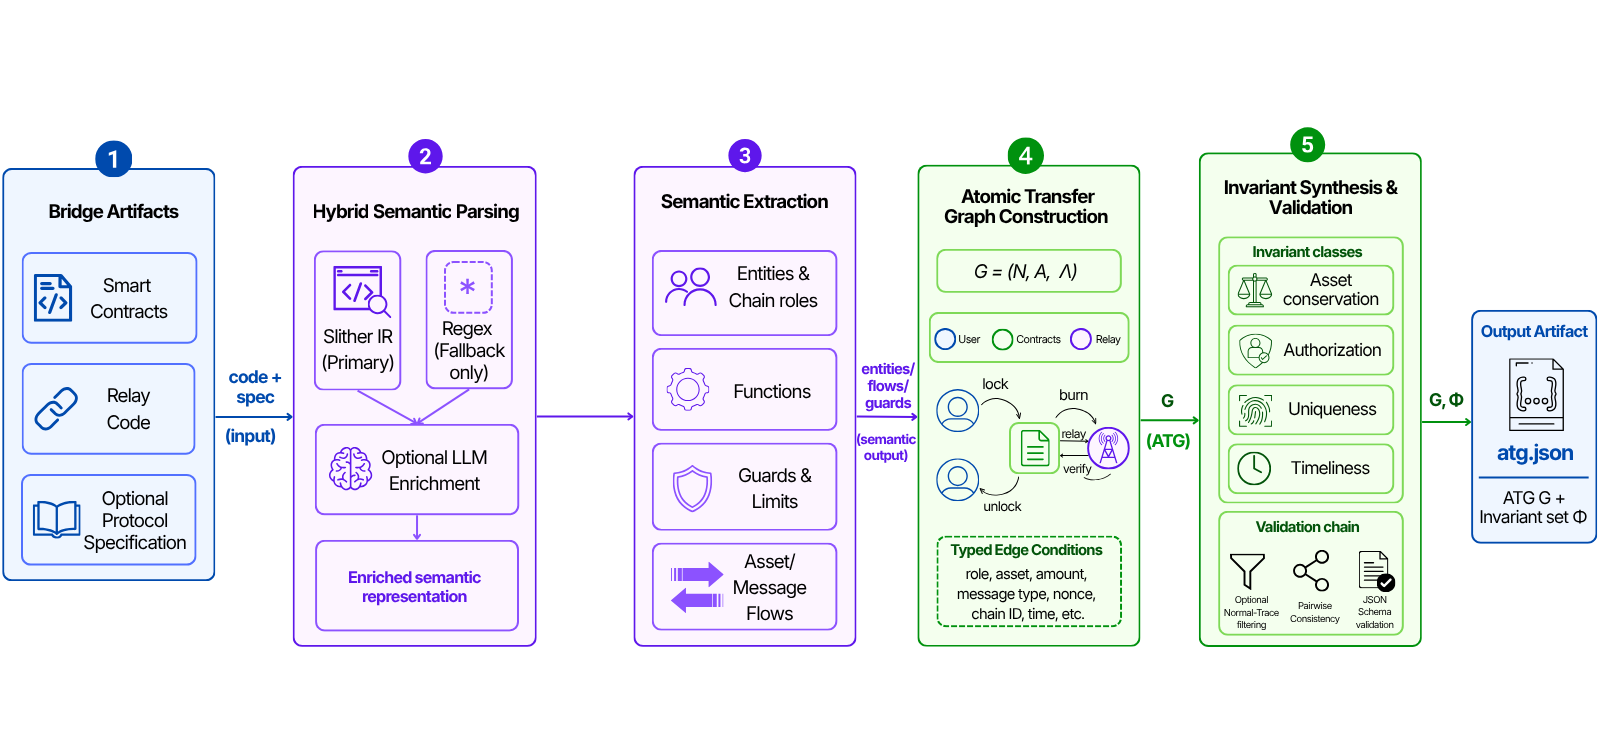
\includegraphics[width=\linewidth]{fig_module1.png}
\caption{Module~1 pipeline. Bridge artifacts are parsed through the Slither IR with a regular-expression fallback and optional LLM enrichment; the semantic representation is compiled into an ATG $G=(N,A,\Lambda)$ and a separate invariant set $\Phi$ covering asset conservation, authorization, uniqueness, and timeliness.}
\label{fig:module1}
\end{figure}

\subsection{Module 2: retrieval-augmented scenario generation}

Module~2 draws on a knowledge base $\mathcal{K}$ of 48 documented cross-chain bridge attacks curated from the SmartAxe and XScope incident collections and the public reports they cite~\citep{liao2024smartaxe, zhang2022xscope}. Each entry records the bridge, date, loss, and affected chains; the vulnerability class, namely access control, fake deposit, reentrancy, signature forgery, initialization flaw, or oracle manipulation; the attack stage on the source chain, off chain, or on the destination chain; the attack trace as a sequence of high-level actions; and the code-level root cause. Entries are embedded with the all-MiniLM-L6-v2 sentence transformer and indexed with the FAISS similarity-search library.

For each invariant $\phi_i \in \Phi$, Module~2 formulates a query that describes $\phi_i$ and the components it involves, retrieves the top-$k$ entries by cosine similarity, and prompts the LLM with the ATG, $\phi_i$, and the retrieved incidents. The LLM adopts the role of a rational adversary and returns an action sequence $S_i = (a_1, \ldots, a_m)$ intended to violate $\phi_i$, together with semantic waypoints $W_i = \{w_1, \ldots, w_p\}$, each a predicate over the execution state that marks an intermediate objective such as an accepted forged message or a consumed nonce. Figure~\ref{fig:module2} shows the transformation from invariants to scenarios and waypoints.

\begin{figure}
\centering
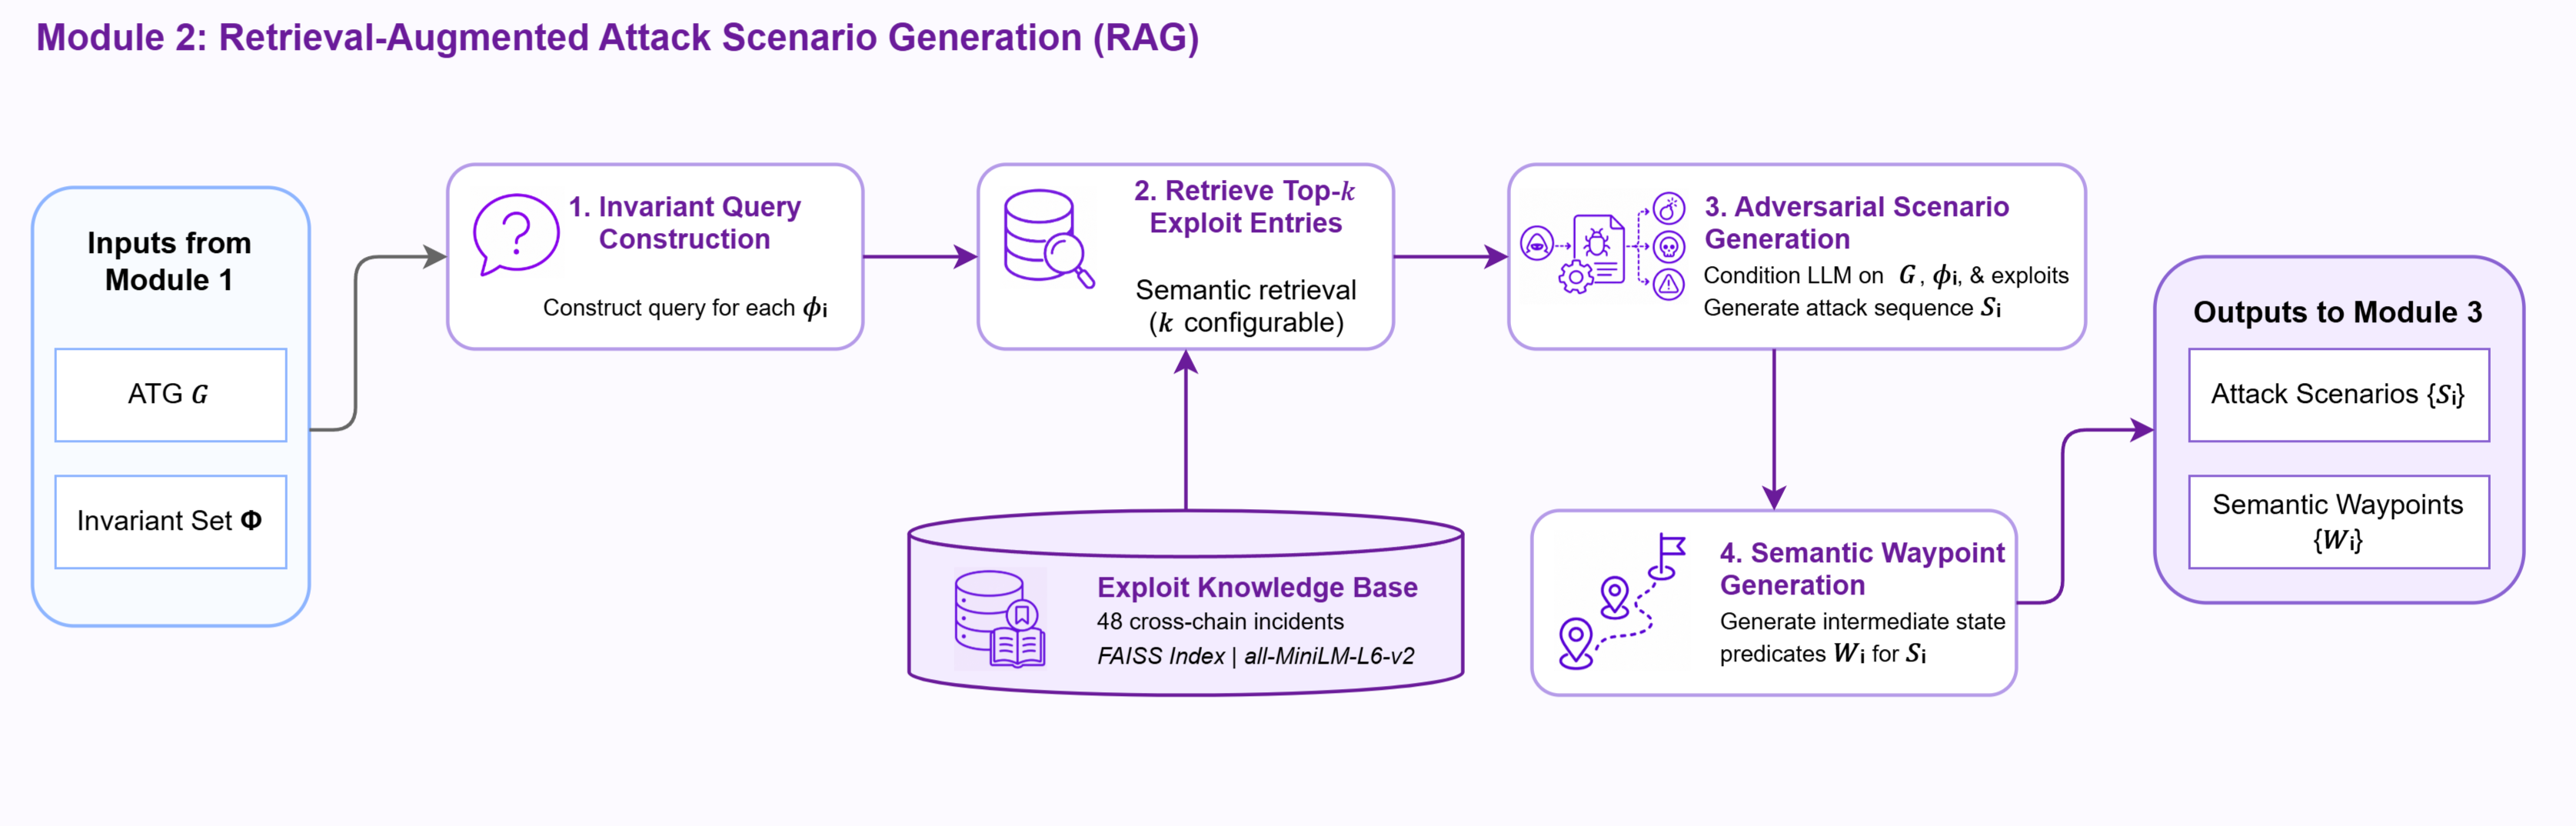
\includegraphics[width=\linewidth]{fig_module2.png}
\caption{Module~2. For each invariant, the module retrieves relevant incidents from the 48-entry knowledge base, generates an adversarial action sequence, and derives semantic waypoints that serve as intermediate objectives for the fuzzer.}
\label{fig:module2}
\end{figure}

\subsection{Module 3: synchronized dual-chain fuzzing}

\paragraph{Dual-EVM environment}
BridgeSentry instantiates two EVM instances, $\text{EVM}_S$ for $\mathcal{C}_S$ and $\text{EVM}_D$ for $\mathcal{C}_D$, each either forked from the target chain at a specified block or started from an empty chain state, and joins them through a mock relay $\mathcal{R}_{\text{mock}}$ under fuzzer control. The relay supports faithful, delayed, tampered, and replayed delivery. Tampering and replay are fault-injection modes whose use Definition~\ref{def:capability} restricts to fixtures that grant the corresponding capability. Figure~\ref{fig:module3} shows the environment.

\begin{figure}
\centering
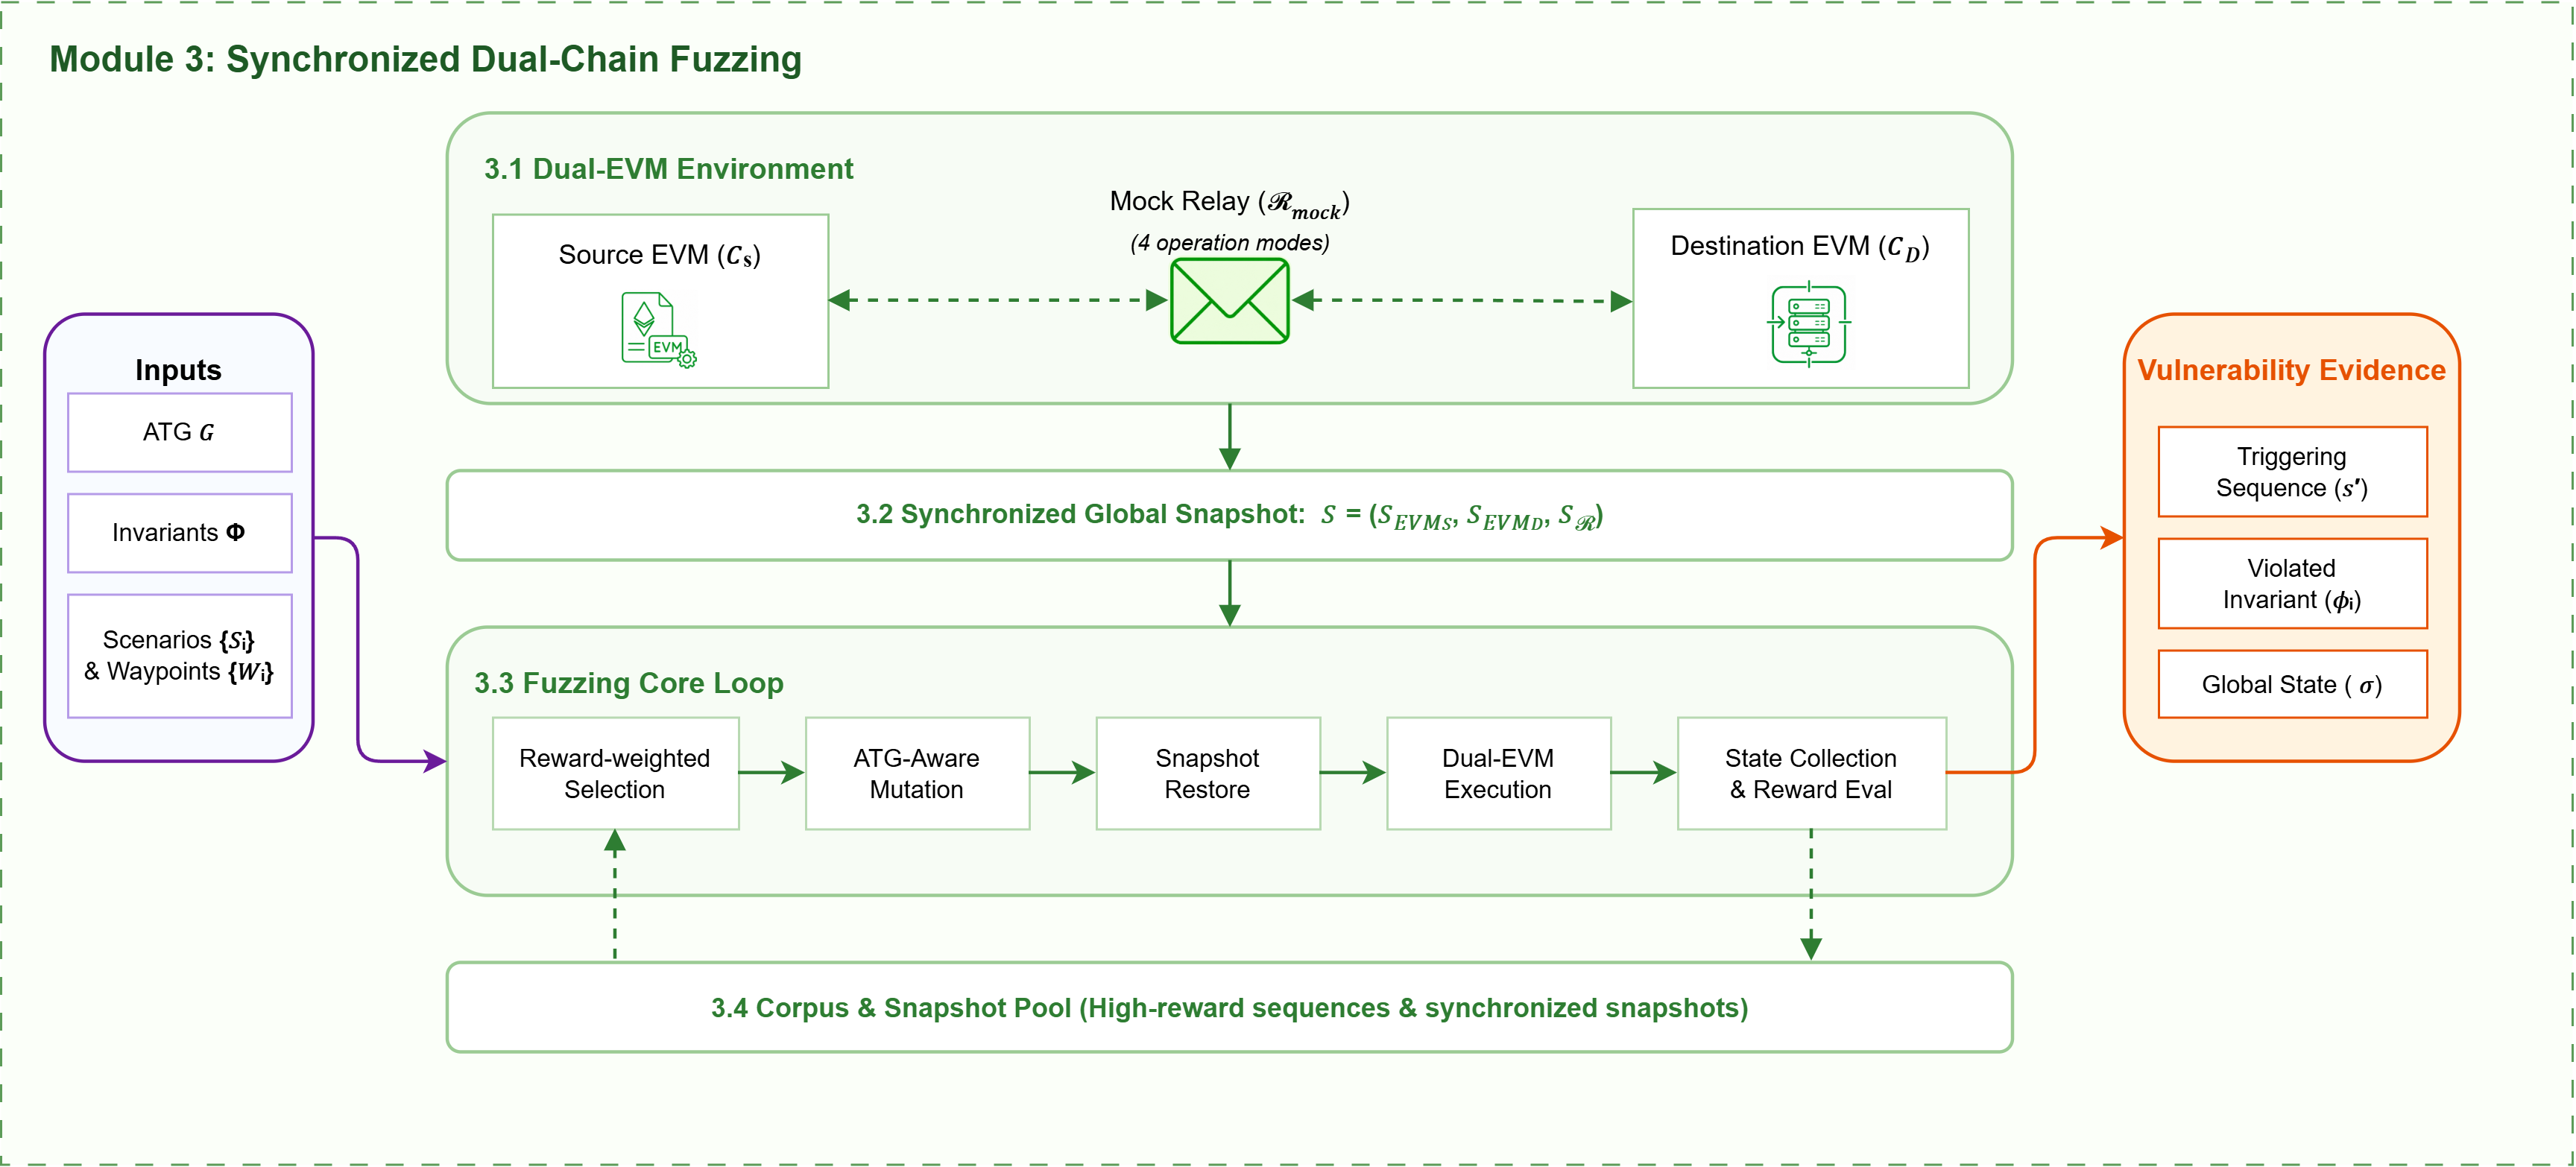
\includegraphics[width=\linewidth]{fig_module3.png}
\caption{Module~3. The source and destination EVM instances interact through the mock relay; a global snapshot captures both EVM states and the relay state, and the fuzzing loop selects, mutates, restores, executes, and scores traces before recording vulnerability evidence.}
\label{fig:module3}
\end{figure}

\paragraph{Global snapshots}
A global snapshot is the triple
\begin{equation}\label{eq:snapshot}
    \mathcal{S} = (S_{\text{EVM}_S}, S_{\text{EVM}_D}, S_{\mathcal{R}}),
\end{equation}
where $S_{\mathcal{R}}$ contains the relay's message queue and its set of processed messages. Capture and restore act on all three components in a fixed order under one global lock. Every restored state is therefore a state that the harness previously reached as a whole, and no explored state pairs a source-chain state with a destination-chain or relay state from a different point of an execution. This property extends the single-chain snapshot reuse of ItyFuzz~\citep{shou2023ityfuzz} to two chains and a relay; it concerns the consistency of harness states and does not model asynchronous finality on live networks.

\paragraph{Waypoint-guided reward}
Instead of code coverage alone, BridgeSentry scores an execution state $\sigma$ by
\begin{equation}\label{eq:reward}
    R(\sigma) = \alpha \cdot \text{cov}(\sigma) + \beta \cdot \frac{|W_{\mathrm{reached}}(\sigma)|}{\max(1,|W|)} + \gamma \cdot \frac{1}{|\Phi|}\sum_{\phi_i \in \Phi}\frac{1}{1+d_i(\sigma)},
\end{equation}
where $\text{cov}(\sigma)$ is normalized code coverage, $W_{\mathrm{reached}}(\sigma)$ is the set of satisfied waypoints, and $d_i(\sigma) \ge 0$ is the distance returned by the checker of $\phi_i$. Each component is clamped to $[0,1]$. The default weights are $\alpha=0.3$, $\beta=0.4$, and $\gamma=0.3$; after every 100 iterations without a new coverage edge, $\alpha$ is multiplied by $0.95$ and the released weight is split equally between $\beta$ and $\gamma$, so that the search relies increasingly on semantic progress once coverage stalls.

For the conservation invariant of Eq.~\eqref{eq:conservation}, let $h_{\kappa} = L_{\kappa} - f_{\kappa} + \delta_{\kappa} - M_{\kappa}$ be the safety margin of transfer $\kappa$ and $q_{\kappa} = \max(1, |L_{\kappa} - f_{\kappa} + \delta_{\kappa}|)$ its scale. The distance is
\begin{equation}\label{eq:distance}
 d_{\text{asset}}(\sigma) =
 \begin{cases}
  0, & h_{\kappa} < 0,\\[2pt]
  1 + h_{\kappa}/q_{\kappa}, & h_{\kappa} \geq 0.
 \end{cases}
\end{equation}
The distance is zero exactly when Eq.~\eqref{eq:conservation} is violated, equals one at safe equality, and decreases monotonically as a safe state approaches the violation boundary. Normalizing by $q_{\kappa}$ keeps the signal comparable across tokens with different decimals and transfer sizes.

\paragraph{Fuzzing loop}
Algorithm~\ref{alg:fuzzing} gives the main loop. Each seed carries a selection weight $w(s)$, initialized to the confidence that Module~2 assigns to its scenario and multiplied by $1 + 0.5\,R(\sigma)$ after each execution that ends in state $\sigma$; a seed admitted during the campaign starts with $w(s) = R(\sigma)$. The capability check rejects a relay tampering or replay mutation before execution unless $C_F$ admits it, and \textsc{SelectSnapshot} chooses the snapshot whose action prefix shares the longest common fingerprint with the mutated seed. The checkers run in the harness process over the collected global state $\sigma$, which contains balances, events, and relay state from both chains.

\begin{algorithm}[!t]
\caption{Dual-chain fuzzing loop of BridgeSentry}
\label{alg:fuzzing}
\begin{algorithmic}[1]
\REQUIRE ATG $G$, invariants $\Phi$, scenarios $\{S_1, \ldots, S_n\}$, waypoints $\{W_1, \ldots, W_n\}$, capability matrix $C_F$, time budget $T$
\ENSURE Set of violation reports $V$
\STATE Initialize $\text{EVM}_S$, $\text{EVM}_D$, and $\mathcal{R}_{\text{mock}}$
\STATE $V \gets \emptyset$; $\text{Corpus} \gets \{S_1, \ldots, S_n\}$
\STATE $\text{SnapshotPool} \gets \{\textsc{CaptureGlobalSnapshot}()\}$
\WHILE{elapsed time $< T$}
    \STATE Select seed $s$ from Corpus with probability proportional to $w(s)$
    \STATE $s' \gets \textsc{Mutate}(s, G)$ \COMMENT{ATG-aware mutation}
    \IF{$\neg\textsc{Admissible}(s', C_F)$}
        \STATE \textbf{continue} \COMMENT{reject inadmissible relay tampering or replay}
    \ENDIF
    \STATE $\textsc{RestoreGlobalSnapshot}(\textsc{SelectSnapshot}(\text{SnapshotPool}, s'))$
    \FOR{each action $(c, f, \text{domain}, \text{params})$ in $s'$}
        \IF{domain $= \mathcal{C}_S$}
            \STATE Execute $f(\text{params})$ on $\text{EVM}_S$
        \ELSIF{domain $= \mathcal{R}$}
            \STATE Process the relay action on $\mathcal{R}_{\text{mock}}$
        \ELSE
            \STATE Execute $f(\text{params})$ on $\text{EVM}_D$
        \ENDIF
    \ENDFOR
    \STATE $\sigma \gets \textsc{CollectGlobalState}()$
    \FOR{each $\phi_i \in \Phi$ with $\phi_i(\sigma) = \text{false}$}
        \STATE $V \gets V \cup \{(s', \phi_i, \sigma)\}$
    \ENDFOR
    \IF{$R(\sigma) > R_{\text{threshold}}$}
        \STATE $\text{Corpus} \gets \text{Corpus} \cup \{s'\}$
        \STATE $\text{SnapshotPool} \gets \text{SnapshotPool} \cup \{\textsc{CaptureGlobalSnapshot}()\}$
    \ENDIF
\ENDWHILE
\RETURN $V$
\end{algorithmic}
\end{algorithm}

\paragraph{ATG-aware mutation}
Mutations follow the structure of the ATG. The mutator reorders actions while respecting the causal dependencies of the graph, substitutes parameters with boundary values, zero values, or values read from on-chain state, inserts calls to functions adjacent in the ATG, switches the relay among faithful, delayed, tampered, and replayed delivery when $C_F$ admits the mode, and advances the block timestamps of $\text{EVM}_S$ and $\text{EVM}_D$ by different increments to expose timing assumptions.

\subsection{Evaluated configuration}\label{sec:evaluated}

The results in Section~\ref{sec:experiments} use an execution-only configuration of Module~3 that implements a subset of the design above. For each fixture, a specification lists the deployment of the vulnerable and the patched contracts on both EVM instances, the pre-incident state (administrators and legitimate user deposits), the relay rule, the pairs of bridged assets, and the root-cause entry point. The relay delivers source-chain events to the destination chain faithfully; tampering and replay are disabled, and the adversary never acts as the relayer. Every trace starts from the same global snapshot, taken after setup. The initial corpus consists either of the Module~2 scenarios, whose actions are mapped to callable functions of the fixture, or of 20 random call sequences. Mutation inserts, removes, and reorders calls and changes their arguments, and a mutated trace enters the corpus when it executes a fixture program counter not executed before.

Several documented bridge exploits need structured arguments that byte-level mutation rarely produces, such as a payload encoded according to the contract application binary interface (ABI) that the receiving contract decodes, or a string that names the function a cross-chain message invokes. The mutator therefore draws arguments from a vocabulary built from the fixture itself: the adversary address and the addresses of the deployed contracts, small integers and boundary amounts, the signatures of the callable functions of the fixture contracts, and the argument values of the initial seeds. From this vocabulary it assembles \texttt{bytes} arguments as ABI encodings of one to four address or amount words and \texttt{string} arguments as function signatures, and random seeds draw their arguments from the same vocabulary. The vocabulary encodes no exploit trace; it contains what an adversary can read from the interfaces and deployment of the fixture. The same mutator is used for every fixture and every seed type.
% TODO(authors): Dict::from_world in official_mode.rs (commit a90aa3d) adds the constant 500000e18 to the amount list. It is the drain amount used by the hand-written exploit tests of five fixtures (FEG, CrossCurve, Ronin 2024, PolyNetwork, Verus), so it leaks the documented exploit into the search. Remove it (or derive amounts from fixture state), re-run the before/after comparison, then confirm the wording "small integers and boundary amounts" above.

This configuration does not use the per-key authorization and uniqueness checkers, the distance of Eq.~\eqref{eq:distance}, the waypoint reward of Eq.~\eqref{eq:reward}, ATG-aware mutation, or relay fault injection, and its oracle does not consume the extracted ATG. These components are part of the design described above; their contribution is not evaluated in this paper.

\section{Evaluation}\label{sec:experiments}

\subsection{Research questions}

The evaluation answers three research questions (RQs).
\begin{itemize}
    \item RQ1, oracle validity: does an invariant-trigger rate distinguish executed exploits from the scenarios that seeded them, and does it fall silent on patched code?
    \item RQ2, valid reconstruction: under Definition~\ref{def:valid}, does BridgeSentry find valid exploits on vulnerable variants and stay silent on patched variants?
    \item RQ3, seed guidance: do retrieval-generated seeds shorten the time to the first valid exploit compared with random seeds?
\end{itemize}
Ablations of semantic extraction, retrieval guidance, and synchronization, parameter sensitivity, and alert burden are not reported; Section~\ref{sec:not-reported} explains why.

\subsection{Benchmark incidents}

Table~\ref{tab:benchmark} lists the incidents used in this paper and the role of each. RQ1 uses the 12 fixtures that an earlier configuration of the harness had built for incidents from 2021 to 2024, drawn from the 48 incidents of the knowledge base. For RQ2 and RQ3, we classified every incident by the root cause reported in public technical analyses. We keep only on-chain incidents, whose root cause is a flaw in a bridge contract and can therefore be confirmed by Definition~\ref{def:valid}. Off-chain incidents, in which the adversary obtained validator or administrator keys, fall outside Definition~\ref{def:valid}, because the evaluated configuration gives the adversary no key-compromise capability. Four incidents are excluded altogether: Wormhole was a flaw in a Solana program, the Socket Gateway exploit involved no cross-chain message, and the GemPad and FEGtoken fixtures modeled neither a bridge nor an incident that a public source confirms.

Three of the earlier incidents are on chain: PolyNetwork, Qubit, and Nomad. We added four on-chain bridge incidents from 2024 to 2026 for which security firms have published technical analyses: the Ronin bridge withdrawal of August 2024, accepted with no operator votes because an initializer of the upgraded contract was never called; the Feed Every Gorilla (FEG) SmartBridge exploit of December 2024, in which a message from an untrusted source extended the list of trusted sources; the CrossCurve exploit of January 2026, in which an express-execution path skipped validation by the message gateway; and the Verus--Ethereum bridge exploit of May 2026, in which a payout was not reconciled with the value exported on the source chain.

For each of the seven on-chain incidents, we wrote an execution specification, which lists the contracts deployed on each chain, the state before the attack, and the relay rule, together with a patched variant. Both are minimal re-implementations of the documented root cause rather than the deployed contracts. A deterministic test replays the documented attack as a sequence of fuzzer actions and checks that it satisfies every condition of Definition~\ref{def:valid} on the vulnerable variant and gains nothing on the patched variant. Two re-implementations simplify the original incident. The Verus source chain, which is not based on the EVM, is replaced by an EVM surrogate, so results for Verus are reported separately. The PolyNetwork keeper is represented as an address, which omits the function-selector collision through which the original attack reached the keeper setter.
% TODO(authors): the PolyNetwork modeling choice (keep the address abstraction or model the selector collision) is still open; update the last sentence when decided.

\begin{table}[!t]
\centering
\caption{Benchmark incidents in chronological order within each group. Root cause: the contract on the source or destination chain of the exploit message that contains the flaw, the off-chain keys that were compromised, or the reason for exclusion. RQ1: the incident has a fixture of the earlier harness configuration, used in RQ1. Spec.: the incident has an execution specification and a patched variant. The year is omitted when no public source confirms the incident as its fixture models it. $^{\dagger}$Source chain replaced by an EVM surrogate.}
\label{tab:benchmark}
\footnotesize
\begin{tabular*}{\linewidth}{@{\extracolsep{\fill}}lrlcc@{}}
\toprule
\hd{Incident} & \hd{Year} & \hd{Root cause} & \hd{RQ1} & \hd{Spec.} \\
\midrule
\multicolumn{5}{@{}l}{\emph{On-chain incidents (used in RQ2 and RQ3)}} \\
PolyNetwork                 & 2021 & Destination-chain contract & Yes & Yes \\
Qubit Finance               & 2022 & Source-chain contract      & Yes & Yes \\
Nomad                       & 2022 & Destination-chain contract & Yes & Yes \\
Ronin bridge (2024)         & 2024 & Destination-chain contract & --- & Yes \\
FEG SmartBridge             & 2024 & Destination-chain contract & --- & Yes \\
CrossCurve                  & 2026 & Destination-chain contract & --- & Yes \\
Verus--Ethereum$^{\dagger}$ & 2026 & Destination-chain contract & --- & Yes \\
\midrule
\multicolumn{5}{@{}l}{\emph{Off-chain incidents (outside Definition~\ref{def:valid})}} \\
Ronin Network (2022)        & 2022 & Off-chain keys             & Yes & --- \\
Harmony Horizon             & 2022 & Off-chain keys             & Yes & --- \\
pGALA                       & 2022 & Off-chain keys             & Yes & --- \\
Multichain                  & 2023 & Off-chain keys             & Yes & --- \\
Orbit Bridge                & 2023 & Off-chain keys             & Yes & --- \\
\midrule
\multicolumn{5}{@{}l}{\emph{Excluded}} \\
Wormhole                    & 2022 & Solana program             & Yes & --- \\
Socket Gateway              & 2024 & No cross-chain message     & Yes & --- \\
GemPad                      & ---  & Not a bridge               & Yes & --- \\
FEGtoken                    & ---  & Not a bridge               & Yes & --- \\
\bottomrule
\end{tabular*}
\end{table}

\subsection{Metrics}

Each run is one campaign of the fuzzer on one fixture variant with one random seed. We report the following measures.
\begin{itemize}
    \item Valid-exploit runs: runs that find at least one trace satisfying Definition~\ref{def:valid}.
    \item Alert runs: runs that find at least one candidate trace with a positive adversary gain. On a patched variant, every alert is a false alarm.
    \item Time to first valid exploit (TTVE): fuzzing-only wall-clock time from the start of the campaign to the first trace that satisfies Definition~\ref{def:valid}. Runs without one are right-censored at the budget, that is, their TTVE is known only to exceed the budget, and a median is reported as $>$\,budget when more than half of the runs are censored.
    \item Unique program counters (PCs): distinct bytecode offsets of the fixture contracts executed during the campaign. This is a measure of code reached, not of basic-block coverage.
    \item Action resolution: the fraction of actions in the Module~2 scenarios that map to a callable function of the fixture.
\end{itemize}

\subsection{Setup}

Module~3 is implemented in Rust on revm, an EVM implementation written in Rust, and orchestration, LLM integration, and retrieval in Python. The reported runs use the configuration of Section~\ref{sec:evaluated} at commit \texttt{df1abb0}, built with the Rust compiler rustc 1.97.0 and the Solidity compiler solc 0.8.20. Both EVM instances query a JSON remote procedure call (JSON-RPC) endpoint that serves an empty chain state, and the fuzzer compiles and deploys the fixture contracts itself, so the runs execute local fixtures rather than forks of mainnet state. The seeds are the scenarios that Module~2 generated with gpt-oss-120b in April 2026, before holdout retrieval was implemented, so retrieval could return the target incident; they were generated for an earlier version of the fixtures. Each configuration, defined by fixture, variant, and seed type, runs with five seeds (1042 to 5042) and a budget of 20\,s, and the full set of configurations was run twice. The runs executed in a cloud container whose hardware allocation was not recorded, so absolute times are indicative only. They predate the argument vocabulary of Section~\ref{sec:evaluated}. A third round repeated the configurations of Table~\ref{tab:official} as batch jobs on a node of a shared computing cluster, with 8 allocated processor cores, 8\,GB of memory, and no graphics processor, using a statically linked build at commit \texttt{ec8f73d} (rustc 1.99.1, solc 0.8.20), which also predates the vocabulary.

\subsection{RQ1: validity of a trigger-rate oracle}\label{sec:rq-oracle}

An earlier configuration of the harness evaluated the LLM-generated invariants with checkers whose global state was assembled from the scenario being executed: the amounts named in the scenario's actions were summed into locked and minted totals, and on-chain balances were added to the state but not read by the checkers. The 229 generated invariants were dispatched by category to three checker functions, each of which mainly tested whether the minted total exceeded the locked total. To test whether this oracle measured execution, we ran it at commit \texttt{db20af7} on all 12 fixtures, with three seeds and a 20\,s budget per fixture and condition, in three conditions: without bytecode execution, so that the checkers saw only scenario-derived state; with the fixture bytecode deployed and executed; and with execution but with every scenario-derived fact removed from the checked state by a diagnostic switch. We also ran a Nomad fixture whose \texttt{acceptableRoot} rejects the zero root, which fixes the documented root cause. Table~\ref{tab:oracle} summarizes the outcome.

\begin{table}[!t]
\centering
\caption{Diagnosis of the earlier trigger-rate oracle (three seeds per fixture, 20\,s each, empty chain state). A fixture counts as triggered when at least one run triggers.}
\label{tab:oracle}
\footnotesize
\begin{tabular*}{\linewidth}{@{\extracolsep{\fill}}p{0.42\linewidth}cp{0.36\linewidth}@{}}
\toprule
\hd{Condition} & \hd{Triggered fixtures} & \hd{Note} \\
\midrule
Scenario-derived state, no bytecode executed & 12/12 & All 36 runs trigger \\
Bytecode executed, scenario-derived state checked & 11/11 & Wormhole not deployable; PolyNetwork 2/3 runs \\
Bytecode executed, execution-derived state only & 0/11 & No run triggers \\
Patched Nomad, scenario-derived state checked & 1/1 & 3 of 3 runs; all 18 invariants violated \\
\bottomrule
\end{tabular*}
\end{table}

When bytecode was executed, the first trigger came after a median of 0.0024\,s (maximum 0.11\,s over the 32 triggering runs), that is, within the first iterations of the campaign, and nine of the eleven deployable fixtures executed no basic block on the destination chain. The trigger rate therefore reflected the generated scenarios rather than the executed code, and the patched Nomad fixture shows that it could not detect a fix. The triggers of the executed condition were bytecode-backed in the sense of Definition~\ref{def:outcomes}, so execution depth alone does not guard against this failure. Results obtained during development with this oracle, including invariant-trigger rates, coverage over the extracted ATG, and module ablations, are withdrawn and not reported.

\subsection{RQ2: valid reconstruction}

Table~\ref{tab:official} reports the first round of the execution-only evaluation. Every vulnerable-variant run found a valid exploit, and no patched-variant run produced a candidate with a positive adversary gain, although each run executed between about 16{,}000 and 55{,}000 traces. The second round, which read the fork block numbers from the fixture metadata instead of using a fixed value, reproduced these outcomes: 5/5 valid-exploit runs in every vulnerable configuration and 0/5 alert runs in every patched configuration. The third round, on the computing cluster, reproduced them again, and none of its 40 runs failed. On these two incidents the patched variant is a working negative control: the oracle that confirms the exploit on the vulnerable variant stays silent once the root cause is fixed. Two incidents are not a benchmark, and the result does not cover off-chain compromises or bridges without an execution specification.

\begin{table*}[!t]
\centering
\caption{Execution-only evaluation, first round (five seeds per configuration, 20\,s each, empty chain state). Module~2 seeds are the retrieval-generated scenarios; random seeds are 20 random call sequences. TTVE: time to first valid exploit; $>$20 marks configurations in which more than half of the runs are censored at the budget.}
\label{tab:official}
\footnotesize
\begin{tabular*}{\textwidth}{@{\extracolsep{\fill}}lllcccccc@{}}
\toprule
\hd{Fixture} & \hd{Variant} & \hd{Seeds} & \begin{tabular}[b]{@{}c@{}}\hd{Valid-exploit}\\ \hd{runs}\end{tabular} & \begin{tabular}[b]{@{}c@{}}\hd{Alert}\\ \hd{runs}\end{tabular} & \begin{tabular}[b]{@{}c@{}}\hd{Median}\\ \hd{TTVE (s)}\end{tabular} & \begin{tabular}[b]{@{}c@{}}\hd{Max}\\ \hd{TTVE (s)}\end{tabular} & \begin{tabular}[b]{@{}c@{}}\hd{Unique}\\ \hd{PCs}\end{tabular} & \begin{tabular}[b]{@{}c@{}}\hd{Actions}\\ \hd{resolved}\end{tabular} \\
\midrule
Nomad & Vulnerable & Module~2 & 5/5 & 5/5 & 0.0089 & 0.0152 & 4,520 & 15/57 \\
Nomad & Vulnerable & Random   & 5/5 & 5/5 & 0.0013 & 0.0017 & 4,520 & --- \\
Nomad & Patched    & Module~2 & 0/5 & 0/5 & $>$20  & ---    & 4,093 & 15/57 \\
Nomad & Patched    & Random   & 0/5 & 0/5 & $>$20  & ---    & 4,093 & --- \\
Qubit & Vulnerable & Module~2 & 5/5 & 5/5 & 0.0040 & 0.0117 & 2,438 & 28/65 \\
Qubit & Vulnerable & Random   & 5/5 & 5/5 & 0.0997 & 0.428  & 2,438 & --- \\
Qubit & Patched    & Module~2 & 0/5 & 0/5 & $>$20  & ---    & 2,487 & 28/65 \\
Qubit & Patched    & Random   & 0/5 & 0/5 & $>$20  & ---    & 2,043 & --- \\
\bottomrule
\end{tabular*}
\end{table*}

\subsection{RQ3: seed guidance}

Module~2 seeds reached the first valid exploit faster than random seeds on Qubit, with a median of 0.0040\,s against 0.0997\,s in the first round and 0.0029\,s against 0.0974\,s in the second, but slower on Nomad, with 0.0089\,s against 0.0013\,s and 0.0056\,s against 0.0011\,s. Random seeds found the exploit within 0.43\,s on both fixtures, so neither fixture can show whether retrieval-generated scenarios help: each has only a few contracts and functions, and coverage-guided mutation reaches the vulnerable entry point almost immediately. Only 15 of 57 Nomad and 28 of 65 Qubit scenario actions mapped to a callable function, partly because the scenarios were generated for an earlier version of the fixtures. A test of semantic guidance needs fixtures with longer exploit sequences, distracting functions, and narrow parameter conditions, together with scenarios generated for those fixtures under holdout retrieval.

\subsection{Results not reported}\label{sec:not-reported}

We do not report an invariant-trigger rate, cross-chain path coverage over the extracted ATG, ablations that remove semantic extraction, retrieval guidance, or synchronized snapshots, parameter sensitivity, or alert burden. Values for these quantities were obtained during development with the oracle of RQ1 and are withdrawn. Execution specifications and patched variants now exist for the seven on-chain incidents, but campaigns on the five incidents other than Nomad and Qubit, with seeds generated for the current fixtures, have not been completed. Holdout retrieval, comparison with BridgeFuzz and single-chain fuzzers, benign bridges, and fixtures with chain reorganizations are likewise not yet evaluated.

\section{Discussion}\label{sec:discussion}

\subsection{Implications for bridge testing}

The main lesson of RQ1 is that, in our harness, the oracle rather than the search determined whether a result meant anything. An oracle that reads its state from the inputs that drive the search reported a perfect trigger rate on every fixture, and execution depth did not expose the problem: in RQ1 most fixtures executed hundreds of target basic blocks on the source chain, yet removing the scenario-derived facts removed every trigger. Two checks are simple to add to an EVM harness and, in our diagnosis, exposed the failure: deriving the checked state only from committed execution, such as token transfer logs, and running every reported trace against a variant in which the documented root cause is fixed. We suggest that bridge-testing tools and benchmarks report both.

Reconstruction under such checks is useful in its own right. An auditor who must confirm that a patch closes a documented exploit, a team that wants a regression test for a past incident, and an investigator who reconstructs how a loss occurred all need an executable trace through the vulnerable contracts that fails on the fixed ones; RQ2 shows this behavior on two incidents.

\subsection{Limitations and threats to validity}

\paragraph{Scope of the evaluation}
The results measure the reconstruction of two documented incidents, Nomad and Qubit; the other five on-chain incidents have specifications but no completed campaign. The scenarios used as seeds were generated with retrieval that could return each target's own incident, and the LLM was pretrained on public post-mortems of the same incidents, so the results do not measure the discovery of unknown vulnerabilities. Leave-one-incident-out, leave-one-family-out, and temporal holdouts, together with a parser-only variant of Module~1 that isolates the contribution of parametric LLM knowledge, are required to assess generalization. Apart from the patched variants, the benchmark has no benign bridges or hard negatives, so it cannot estimate a false-positive rate on unrelated code.

\paragraph{Evaluated subset of the design}
The evaluated configuration exercises dual-EVM execution, faithful relay delivery, restoration of a global snapshot, Module~2 scenarios as seeds, coverage-guided mutation, and an adversary-side conservation check. The per-key authorization and uniqueness invariants, the distance-guided waypoint reward, ATG-aware mutation, relay fault injection under the capability matrix, and the use of extracted ATGs by the oracle are design elements whose contribution remains unmeasured.

\paragraph{Comparison with other tools}
We do not report a head-to-head comparison with BridgeFuzz~\citep{winkler2026bridgefuzz} or with single-chain fuzzers. A fair comparison requires adapting every fixture to each tool's deployment model under a common budget and hardware allocation, and single-chain fuzzers can at most exercise one side of each exploit because they cannot execute the relay step. Such a study, on the fixtures that each tool supports, is the most direct test of whether transfer-key oracles and retrieval guidance outperform coverage-guided bridge fuzzing.

\paragraph{Fixture fidelity}
The specifications of the on-chain incidents are minimal re-implementations of the documented root causes rather than the deployed contracts, and the runs used local fixtures on an empty chain state rather than forks of mainnet state. The Verus re-implementation replaces a source chain that is not based on the EVM with an EVM surrogate, and the PolyNetwork re-implementation represents the keeper as an address. The five off-chain incidents are compromises of validator or administrator keys and fall outside Definition~\ref{def:valid}. Module~1 requires Solidity source, so bridges written in Vyper, Huff, or Yul must first be compiled to Solidity-compatible interfaces.

\paragraph{Oracle validity}
The adversary-side conservation check detects exploits that move bridged value to the adversary; a violation of authorization or uniqueness that produces no net gain for the adversary would be missed. The extracted invariants have no independently labeled ground truth, and an LLM may propose an invariant that is wrong or vacuous; integrating verification of candidate invariants, for instance through INVCON+~\citep{liu2025invcon}, would address this risk.

\paragraph{Synchronization}
Global snapshots guarantee consistent harness states but cannot represent asynchronous block production, variable finality, or reorganizations on live networks. No reported result depends on them beyond restoring the initial state; their benefit can appear only on fixtures that roll back one chain while the other advances, such as a destination-chain rollback that invalidates a delivered message after the source chain has finalized a later transfer.

\paragraph{Statistics and cost}
Each configuration ran with five seeds in each of two rounds; medians, maxima, and censored runs are reported, but statistical comparisons need more seeds per configuration and survival estimates that treat runs without a valid exploit as censored observations~\citep{klees2018evaluating}. The hardware allocation of the runs was not recorded. End-to-end latency including extraction and generation, LLM cost, and parsing failure rates were not recorded in a reportable form.

\section{Conclusion}\label{sec:conclusion}

This paper presented BridgeSentry, a dual-EVM fuzzing harness for reconstructing cross-chain bridge exploits, whose design makes the canonical transfer key the unit of its oracle and guidance, and whose evaluated configuration uses retrieval-generated attack scenarios to seed the search. Its main empirical finding concerns evaluation: an oracle that derived its state from the generated scenario text reported violations on all 12 historical fixtures without executing target code, on none once restricted to execution-derived state, and still on a patched fixture. Under an execution-only criterion with paired patched variants, BridgeSentry found a valid exploit in every vulnerable-variant run and raised no alert in any patched-variant run of the Nomad and Qubit fixtures, while retrieval-generated seeds were not consistently faster than random ones on these small fixtures. These results suggest that bridge-testing tools be judged by oracles that read only executed state and by patched-variant controls rather than by trigger rates.

Future work will run campaigns on the five on-chain incidents whose specifications and patched variants are complete and add harder incidents, regenerate scenarios for them under incident-, family-, and time-disjoint retrieval, evaluate the per-key authorization and uniqueness checkers and the waypoint reward that the current evaluation does not exercise, compare BridgeSentry with BridgeFuzz and single-chain fuzzers on a common fixture set, and add fixtures with chain reorganizations and finality reversion that exercise synchronized snapshots.

\section*{Declaration of generative AI and AI-assisted technologies in the manuscript preparation process}
During the preparation of this work the authors used Gemini and OpenAI Codex to improve language clarity and to support editorial revision. After using these tools, the authors reviewed and edited the content as needed and take full responsibility for the content of the published article.

\section*{Declaration of competing interest}
The authors declare that they have no known competing financial interests or personal relationships that could have appeared to influence the work reported in this paper.

\section*{Funding}
This research did not receive any specific grant from funding agencies in the public, commercial, or not-for-profit sectors.

\section*{Data availability}
The source code, prompt templates, knowledge-base snapshot, fixture metadata, and raw results will be made available on request. The project repository is not linked in this manuscript to preserve double-anonymized review.

\bibliographystyle{cas-model2-names}
\bibliography{references}

\end{document}
